\begin{figure}[tbp]
\centering
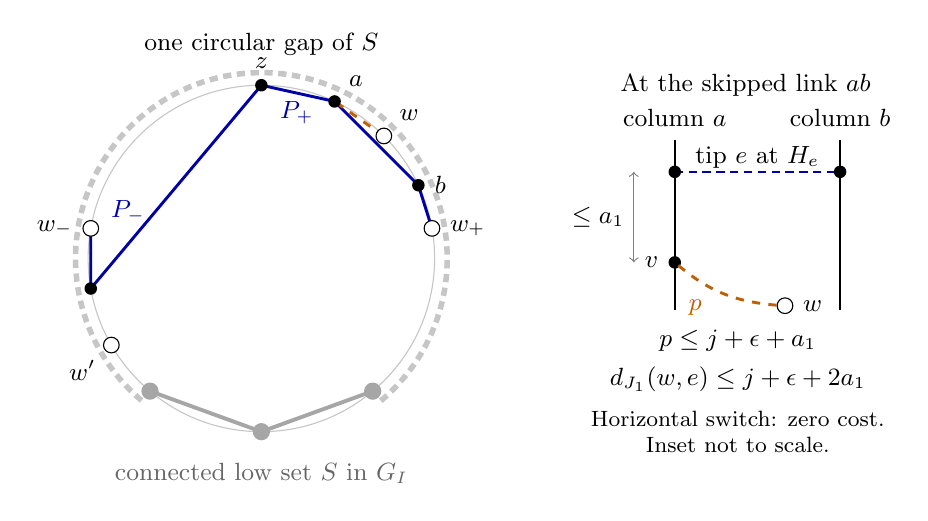
\begin{tikzpicture}[x=1cm,y=1cm,font=\small,
  vertex/.style={circle,fill=black,inner sep=1.6pt},
  seed/.style={circle,draw=black,fill=white,inner sep=2pt},
  low/.style={circle,fill=gray!70,inner sep=2.2pt}]
  \draw[gray!45] (0,0) circle (2.2);
  \draw[gray!45,densely dashed,line width=2pt] (310:2.36) arc (310:590:2.36);
  \node[align=center,fill=white,inner sep=2pt] at (0,2.72) {one circular gap of $S$};
  \coordinate (z) at (90:2.2);
  \coordinate (wm) at (170:2.2);
  \coordinate (q) at (190:2.2);
  \coordinate (wp) at (10:2.2);
  \coordinate (a) at (65:2.2);
  \coordinate (b) at (25:2.2);
  \coordinate (w) at (45:2.2);
  \coordinate (partner) at (210:2.2);
  \coordinate (s1) at (230:2.2);
  \coordinate (s2) at (270:2.2);
  \coordinate (s3) at (310:2.2);
  \draw[gray!70,line width=1.4pt] (s1)--(s2)--(s3);
  \draw[blue!65!black,line width=1.05pt] (z)--node[left,pos=.62] {$P_-$} (q)--(wm);
  \draw[blue!65!black,line width=1.05pt] (z)--(a)--(b)--(wp);
  \node[blue!65!black] at (.45,1.85) {$P_+$};
  \draw[orange!75!black,dashed,line width=1.05pt] (w)--(a);
  \node[vertex,label=above:$z$] at (z) {};
  \node[seed,label=left:$w_-$] at (wm) {};
  \node[vertex] at (q) {};
  \node[seed,label=right:$w_+$] at (wp) {};
  \node[vertex,label=above right:$a$] at (a) {};
  \node[vertex,label=right:$b$] at (b) {};
  \node[seed,label=above right:$w$] at (w) {};
  \node[seed,label=below left:$w'$] at (partner) {};
  \foreach \s in {s1,s2,s3} {\node[low] at (\s) {};}
  \node[gray!80!black,below] at (0,-2.48) {connected low set $S$ in $G_I$};

  \begin{scope}[shift={(5.25,.05)}]
    \node[align=center] at (.9,2.15) {At the skipped link $ab$};
    \draw[thick] (0,-.7)--(0,1.45);
    \draw[thick] (2.1,-.7)--(2.1,1.45);
    \node[above] at (0,1.5) {column $a$};
    \node[above] at (2.1,1.5) {column $b$};
    \draw[blue!65!black,densely dashed,line width=.9pt] (0,1.05)--(2.1,1.05);
    \node[above,fill=white,inner sep=1pt] at (1.05,1.05) {tip $e$ at $H_e$};
    \node[vertex] at (0,1.05) {};
    \node[vertex] at (2.1,1.05) {};
    \node[vertex,label=left:$v$] at (0,-.1) {};
    \node[seed,label=right:$w$] (wi) at (1.4,-.65) {};
    \draw[orange!75!black,dashed,line width=1.05pt] (wi) to[bend left=18] node[below left,pos=.6] {$p$} (0,-.1);
    \draw[<->,gray] (-.52,-.1)--node[left,black] {$\le a_1$} (-.52,1.05);
    \node[align=center] at (.8,-1.35) {$p\le j+\epsilon+a_1$\\[3pt]$d_{J_1}(w,e)\le j+\epsilon+2a_1$};
    \node[align=center,font=\footnotesize] at (.8,-2.25) {Horizontal switch: zero cost.\\Inset not to scale.};
  \end{scope}
\end{tikzpicture}
\caption{The key step in Proposition~\ref{pack:bound}, shown for a
surviving seed $w$. In a gap of the connected low set $S$, an extreme
path skips the column of $w$ by the terminal link $ab$. The witness
partner $w'$ is outside the small ball and lies strictly outside the
closed interval $[a,b]$.
The descending path from $w$ must first reach $a$ or $b$; call that point
$v$. Only this first prefix is shown in orange dashes.
Survival of the low-tip test gives $s(e)\ge s(w)-j$, forcing the
short prefix estimated in the inset. Blue paths use $G_{J_2}$; connections
of $S$ may use the larger graph $G_I$. The circular drawing records column
order, not metric lengths; extreme paths need not be monotone in that order.}
\label{fig:surviving-seeds}
\end{figure}
